\section{Embedded Peripherals}
\begin{minipage}{0.4\linewidth}
    \subsection{Interrupts \embsys{299}{7.1}}
    \begin{itemize}
    	\item A signal indicating an event, which needs immediate CPU attention
    	\item More efficient event handling than polling
    	\item IRQ $\rightarrow$ Interrupt Service Request
    	\item ISR $\rightarrow$ Interrupt Service Routine
    	\item SRQ $\rightarrow$ Service Request
    \end{itemize}
\end{minipage}
\begin{minipage}{0.5\linewidth}
    \subsubsection{Interrupt Triggers}
    \begin{tabular}{ll}
    	\textbf{Hardware Trigger}& Rising-Edge, Falling-Edge, Logic Level\\
    	\textbf{Software Trigger}& Software Event in Userprogram\\
    	\textbf{CPU Exception}& CPU State, Divison by Zero, Overflow etc.\\
    \end{tabular}
\end{minipage}

\subsubsection{Maskable vs Non-maskable Interrupt}
\begin{tabular}{ll}
	\textbf{Maskable Interrupt}& Can be blocked through the GIE flag\\
	& Most commen Type of interrupt\\
	\textbf{Non-maskable Interrupt (NMI)}& Cannot be blocked, always served\\
	& Reserved for system critical events\\
\end{tabular}



\begin{minipage}{11cm}
        \subsubsection{Interrupt Identification Method \embsys{300}{7.1.1}}
    \begin{itemize}
		\item \textbf{Non-vectored Interrupt}
		\subitem Single Interrupt Line
		\subitem Single ISR for all devices
		\subitem CPU identifies source by polling service request (SRQ) flags
    \end{itemize}
\end{minipage}	
	\begin{minipage}{8cm}
		\hspace{0.5cm}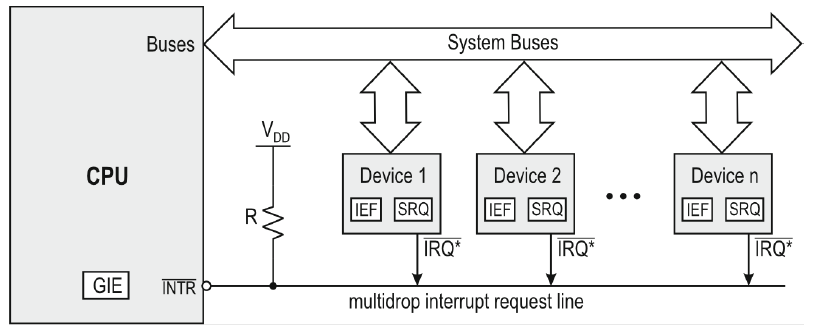
\includegraphics[width=7cm]{images/nonvectored.png}
	\end{minipage}
	\begin{minipage}{11cm}
            \begin{itemize}
		\item \textbf{Vectored Interrupt}
		\subitem Require an interrupt Acknowledgment (INTA) cycle
		\subitem Interface generate an ID number (vector) upon INTA
		\subitem ID Number allows calculating ISR location
    \end{itemize}
	\end{minipage}
		\begin{minipage}{8cm}
		\hspace{0.5cm}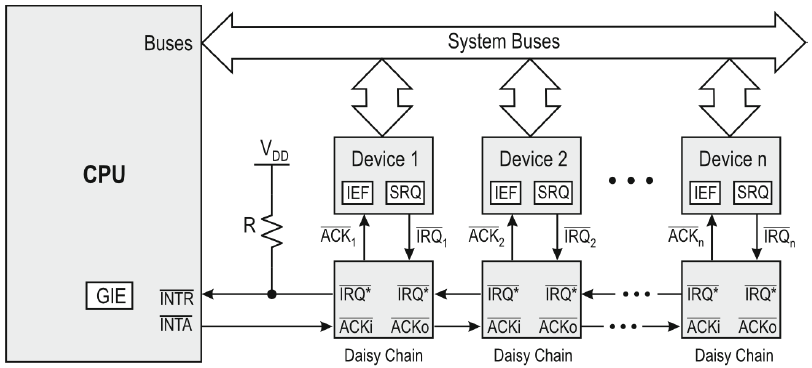
\includegraphics[width=7cm]{images/vectored.png}
	\end{minipage}
    \begin{itemize}
	\item \textbf{Auto-vectored}
	\subitem Each device has a fixed vector or ISR adress
	\subitem No INTA cycle or vector issuing required
	\subitem CPU loads direct ISR address into PC to execute ISR
\end{itemize}

\begin{minipage}{0.6\linewidth}
    \subsubsection{Interrupt Priority Handling \embsys{306}{7.1.5}}
    \begin{itemize}
    	\item Non-vectored Interrupt
    	\subitem Polling order of SRQ flags decides priority
    	\item Vectored Interrupt
    	\subitem Daisy-Chain:All devices in serie. The closer the device to the CPU the higher the priority
    	\subitem Interrupted Controlled: Uses central arbiter for resolving priorities
    \end{itemize}
\end{minipage}
\begin{minipage}{0.5\linewidth}
    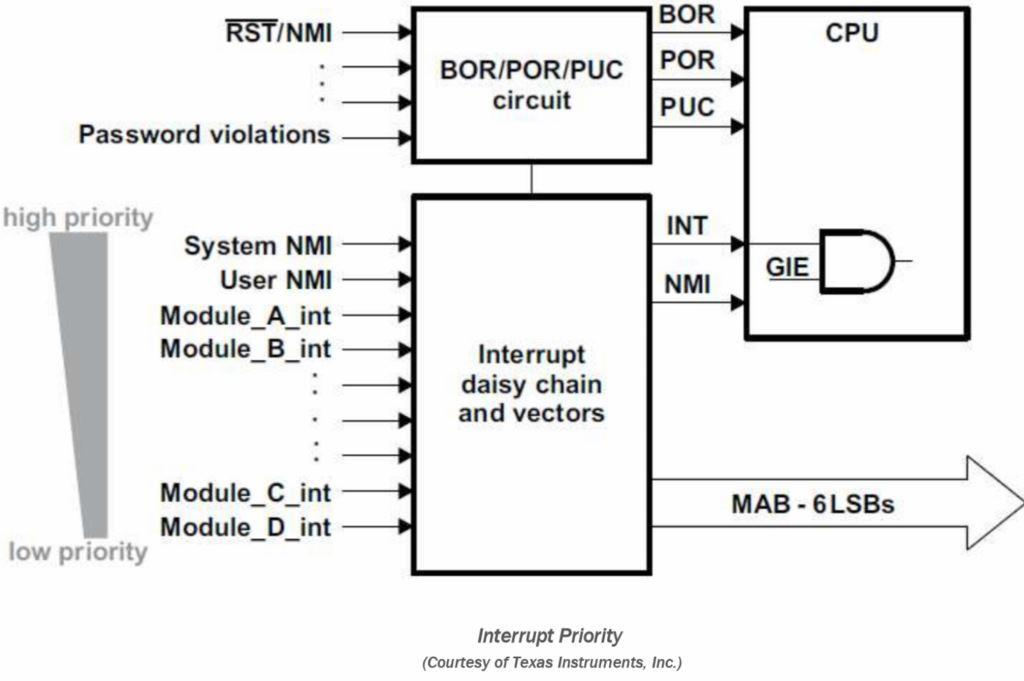
\includegraphics[width=0.9\linewidth]{images/ISRPrio}
\end{minipage}
\clearpage
\pagebreak
%===========================================================
\subsubsection{Interrupt Service Sequence \embsys{303}{7.1.3}}
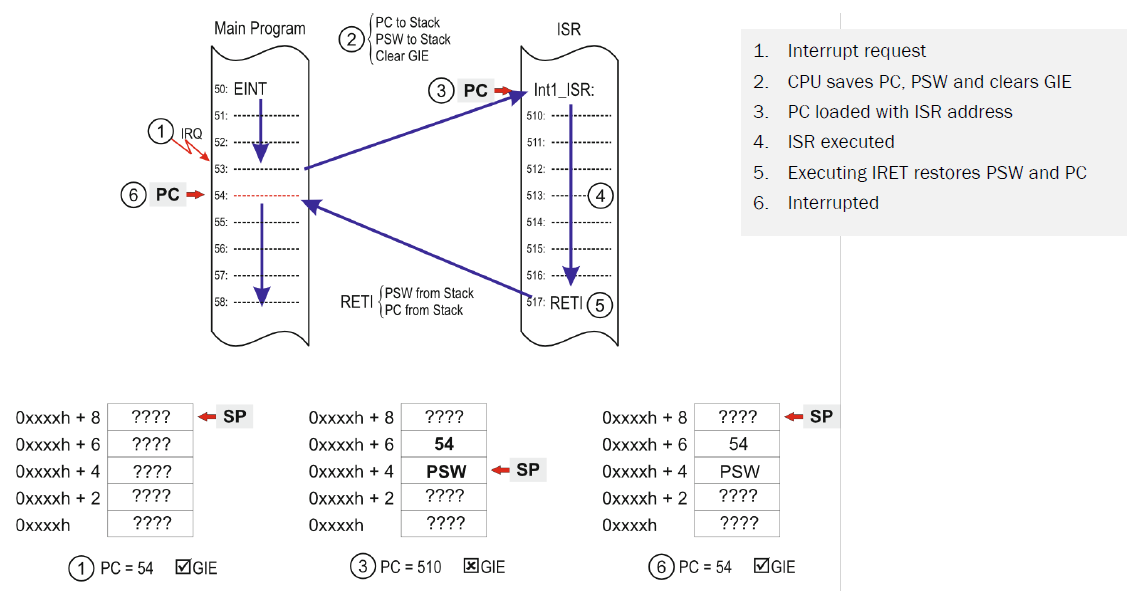
\includegraphics[width=16cm]{images/iss.png}

\subsection{Interrupthandling in the MSP430 \embsys{310}{7.2}}
\begin{itemize}
    \item Auto-vectored and Daisy-Chain
    \item System Resets: Highest priority, non-maskable, triggerd by Watchdog, Power-UP
    \item Non-maskable: Cannot be masked through GIE-Flag, but masked through their own flag, triggerd by oscillator fault, flash key access violation
    \item Maskable: all other sources than reset \& NMI, masked by GIE-Flag, fixed priorities
\end{itemize}
\subsubsection{System Reset}



\subsection{Interrupt Software Design \embsys{7.3}{315}}


\subsection{Timers and Event Counters \embsys{330}{7.4}}
\subsubsection{Timer Structure}
A Binary Counter Driven by a Periodic Signal.It is possible to cascade multiple counters\\
\vspace{1cm}
\begin{minipage}{9cm}
	\begin{itemize}
		\item Mux -> Clock Source selector
		\item Prescaler -> Clock frequency divider
		\item Counter -> n-bit binary counter
		\item Comparator -> compares Counter Output with Compare Register
	\end{itemize}
\end{minipage}
\begin{minipage}{10cm}
	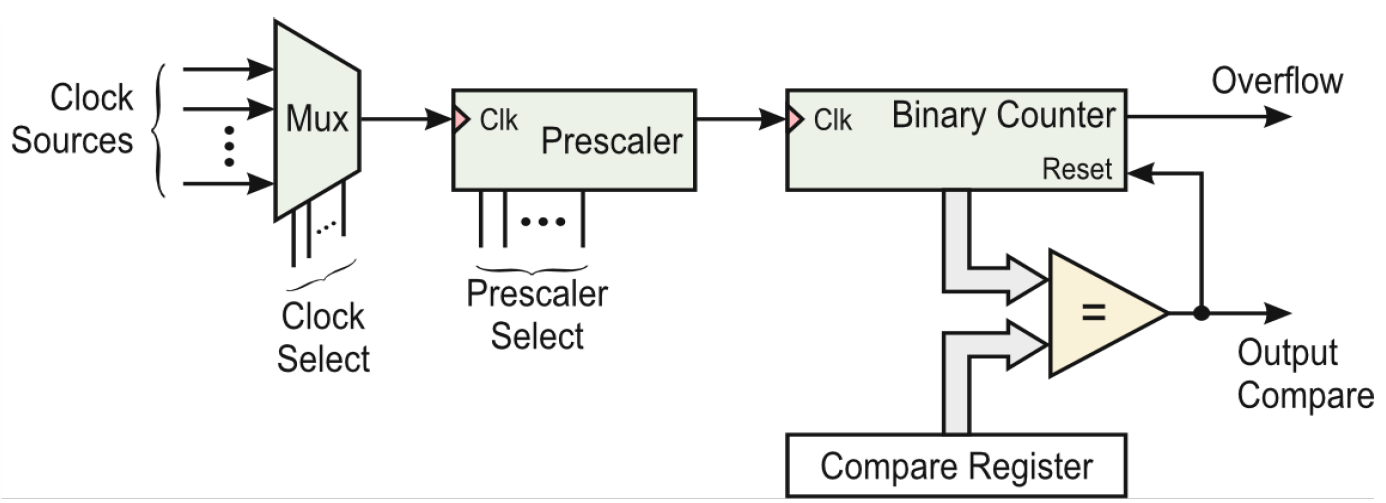
\includegraphics[width=10cm]{images/timerstructure.png} 
\end{minipage}
\begin{multicols}{2}
	\subsubsection{Interval Timer vs Event Counter}
	\begin{itemize}
		\item \textbf{Interval Timer}
		\subitem Measures the time elapsed after k clock cycles
		\item \textbf{Event Counter}
		\subitem Counts the occurrence of k external events
	\end{itemize}	
	\subsubsection{Timer Application}
	\begin{itemize}
		\item Watchdog Timers (WDT)
		\item Realtime Clocks (RTC)
		\item Baud Rate Generator (BRG)
		\item Pulse-Width Modultation (PWM)
	\end{itemize}
\end{multicols}

\textbf{Signature Timer Application \embsys{336}{7.4.3}}\newline
\begin{tabular}{p{5cm} p{15cm}}
	\textbf{Watchdog Timer } &
    Monitor Events within an expiration intervals\newline
	 If WDT expires before the event occurs, a default action is executed\newline
	 If the event occurs within the defined interval, cancel and restart WDT\newline
	 In MSP430 the WDT is 16-Bit (MaxCount: $2^{16}=32'768$) \newline
	 and configure over Register WDTTMSEL\\
     
	\textbf{Realtime Clocks} &
    32-bit Timer with selectable Clock-Source\newline
    Can be used as calendar or counter (H.Min.Sec)\newline
    The accuracy depend greatly on the used Cristal\\
    
	\textbf{Baud Rate Generator} &
     $ \text{Baud Rate}=\dfrac{f_{clk}}{PS \cdot TopCount} $\newline
     PS=Prescaler Value \quad TC= Compare Value\newline
     Directly impacts Bit Time on serial communication\\
     
	\textbf{Pulse-Width Modulation} &
    Produces a Signal which duty cycle is controlled by the MCU \newline
    $ \text{duty cycle}=\dfrac{t_{high}}{T} $\\
\end{tabular}


\clearpage
\pagebreak